\documentclass[journal]{IEEEtran}

\usepackage[pdftex]{graphicx}
\DeclareGraphicsExtensions{.png}

\usepackage{cite}
\usepackage{setspace}
\usepackage{amsmath}
\usepackage{hyperref}


\begin{document}

\title{CSCI 580 : Monte Carlo Path Tracing}
\markboth{Thursday~December~3\textsuperscript{rd}~2015}
{December~3\textsuperscript{rd}~2015}
\author{
	Sincennes, Alexandre
	\texttt{sincenne@usc.edu}\\
	\and
 	Peechankottil Manikandan, Sajini
 	\texttt{smanikan@usc.edu}\\
  	\and
	Guanzhou Liu, Vincent
 	\texttt{guanzhol@usc.edu}\\
  	\and
	Ramirez, Bernie
 	\texttt{berniera@usc.edu}\\
  
}
\maketitle

%===================================================

\section{Abstract}
This will depend on our results.\\
I predict this paper to be around 4 pages since it's in a rather condensed format.

%===================================================

\section{Introduction}
Rendering via the use of rays, such as in the Monte Carlo path tracing approach, stands in stark contrast to the rasterization of triangles, which is the faster and more common approach to rendering, and the one used throughout the assignments of the CSCI 580 course. However, with path tracing it is possible to achieve photorealism by simulating the travel of light, which bounces off surfaces, resulting in shadows, specular as well as diffuse reflections andrefractions rather than the surface shading approach used in renderers that make use of rasterization.

%===================================================

\section{Prior Work}
The origins of path tracing begin with ray tracing, first outlined in A. Appel's 1968 paper[1]. In the ray tracing technique, rays are cast out from the camera, or eye, through the image plane, and into the scene. The first surface it collides with is the one rendered for that pixel. Additionally, rays called shadow rays are cast from the light sources and determine whether or not the surface is being occluded by another, which would be collided with first by the shadow ray. A further development was Whitted ray tracing[2], wherein rays generate new rays upon collision with a surface, for direct illumination, perfect refraction and perfect reflection.

\par

Also instrumental for Monte Carlo path tracing was work in radiosity, which takes into account lighting emitted from diffuse surfaces rather than specular reflection. J. Kajiya's 1986's paper[3] on the rendering equation brings a mathematical basis for these relationships, described by:

\begin{center}
$L_{\text{o}}(\mathbf x,\, \omega_{\text{o}},\, \lambda,\, t) \,=\, L_e(\mathbf x,\, \omega_{\text{o}},\, \lambda,\, t) \ +\, \int_\Omega f_r(\mathbf x,\, \omega_{\text{i}},\, \omega_{\text{o}},\, \lambda,\, t)\, L_{\text{i}}(\mathbf x,\, \omega_{\text{i}},\, \lambda,\, t)\, (\omega_{\text{i}}\,\cdot\,\mathbf n)\, \operatorname d \omega_{\text{i}}$
\end{center}

\begin{flushright}
\par 
(1)
\end{flushright}

\par
Monte Carlo path tracing combines the techniques of reflected or refracted rays by recursively generating other rays, but also captures the lighting relations between diffuse surfaces. Using random numbers, it approximates the integration found the rendering equation by using the Russian Roulette technique for the generation of every new ray, i.e. a random number between zero and one is generated and compared to its colour coefficients.

\section{The Monte Carlo Path Tracing Algorithm}
The essentials of the Monte Carlo algorithm are surprisingly simple and can be summed as thus[4]:

\begin{description}
  \item[1)] Generate a ray from the camera (position x,y, horizontal and vertical fields of view u,v), passing through the image plane, with $weight = 1$
  \item[2)] Find the point of intersection with the nearest surface
  \item[3)] Randomly (Russian Roulette) decide whether the light is emitted or reflected (test against this random number against the Kd of the surface):
  \item[3A)] if emitted, return $weight * shading$ from light source(s)
  \item[3B)] if reflected, $weight \mathrel{*}= Ks$, randomly scatter the ray according to a probability density function (pdf) approximating its bidirectional refletance distribution function (brdf), and go to step 2
\end{description}

In order for this algorithm to be implemented, other algorithms such as ray-triangle intersection and Phong shading (for emitted light) must also be implemented. 
Additionally, a BRDF pdf must be created for each surface. A reasonable BRDF pdf would be a uniform distribution, wherein \emph{any} 
vector (x,y,z) which is in the hemisphere of the surface is randomly selected.

\section{Application Structure}
Firstly, we used the codebase of the previous assignments as a launching point for the project. Thus, the GUI and initialization, as well other elements such as the rendering parameters, the functions for displaying pixels to the screen and a number of vector and matrix functions were borrowed directly from previous assignments. However, rasterization-related functionality was thrown out and replaced with an entirely new way of rendering via rays.

\section{Graphics Pipeline}
The graphics pipeline was designed as follows: initialization is carried out, wherein global properties such as camera position and lights are defined. Then, the meshes are loaded into memory as a data structure encompassing all triangles. Each vertex in the triangle has a position, a normal, as well as information on their specular, diffuse and ambient coefficients, which differs from the global Ks, Kd and Ka found in the assignment renderer. Next, this set of all geometry is used by the path tracing technique to determine colour at each pixel, which is finally fed to the same display as the one used in previous asignments.

\section{The Path Tracing Implementation}

\begin{figure}[!t]

\centering
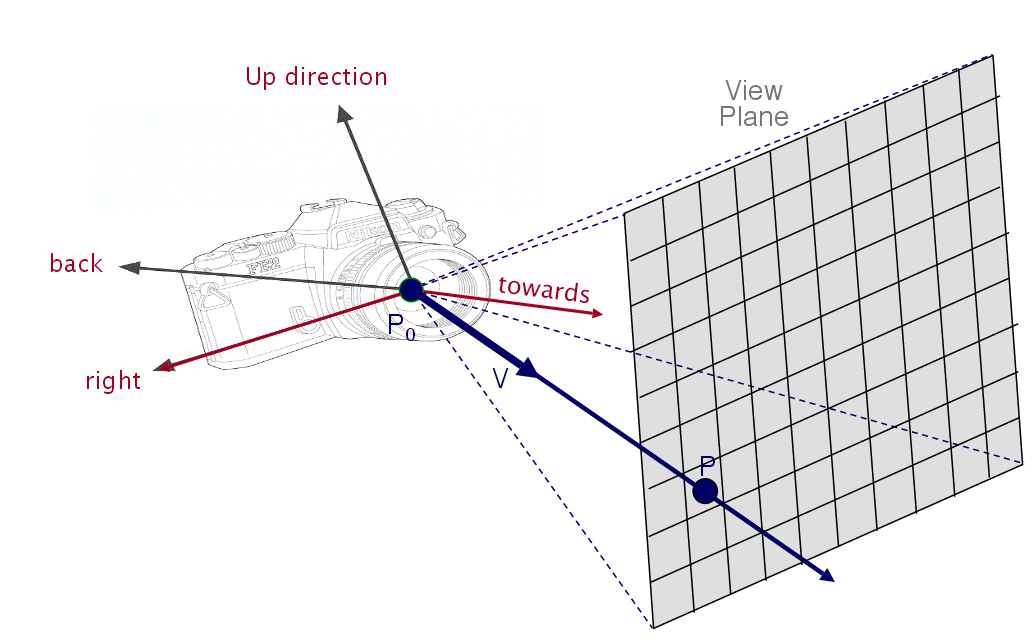
\includegraphics[width=2.5in]{raycast_viewplane}
\caption{Casting a ray through the image plane}
\label{raycast_viewplane}

\end{figure}

\section{Results}
Pictures, maybe some figures for different numbers of rays.

\section{Challenges \& Observations}


%===================================================

\begin{thebibliography}{4}

\bibitem{Appel}
Appel, A. Some techniques for shading machine renderings of solids. \emph{AFIPS '68 (Spring) Proceedings of the April 30--May 2, 1968, spring joint computer conference}:37-45, 1968.

\bibitem {Whitted}
Whitted, T. An improved illumination model for shaded display. \emph{Comunications of the AMC}, 23(6):343-349, 1980.

\bibitem {Kajiya}
Kajiya, J. The Rendering Equation. \emph{SIGGRAPH '86}, 20(4):143-150, 1986.

\bibitem {Chapter}
\url{http://cs.brown.edu/courses/cs224/papers/mc_pathtracing.pdf} page 9

\end{thebibliography}

%===================================================

\end{document}
